%% LaTeX-Beamer template for KIT design
%% by Erik Burger, Christian Hammer
%% title picture by Klaus Krogmann
%%
%% version 2.1
%%
%% mostly compatible to KIT corporate design v2.0
%% http://intranet.kit.edu/gestaltungsrichtlinien.php
%%
%% Problems, bugs and comments to
%% burger@kit.edu

\documentclass[18pt]{beamer}
\usepackage[utf8x]{inputenc}
\usepackage{units}
\usepackage{booktabs}

%% CUSTOM
\usepackage{amsmath}
\usepackage{algpseudocode}

%% Definitions
\DeclareMathOperator{\div2}{div}
\renewcommand{\algorithmicrequire}{\textbf{Input:}}
\renewcommand{\algorithmicensure}{\textbf{Output:}}
\algnewcommand\algorithmicto{\textbf{to}}
\algrenewtext{For}[3]{\algorithmicfor\ $#1 \gets #2$ \algorithmicto\ $#3$ \algorithmicdo}
\algnewcommand\algorithmicod{\textbf{od}}
\algrenewtext{EndWhile}{\algorithmicod}
\algrenewtext{EndFor}{\algorithmicod}
%\AtBeginSection[]{%
%\begin{frame}<beamer> % do nothing in handouts
%    \frametitle{Überblick}
%    \tableofcontents[sectionstyle=show/shaded,
%    subsectionstyle=show/show/hide]
%\end{frame}
%}
%\AtBeginSubsection[]{%
%\begin{frame}<beamer> % do nothing in handouts
%    \frametitle{Überblick}
%    \tableofcontents[sectionstyle=show/shaded,
%    subsectionstyle=show/shaded/hide]
%\end{frame}
%}

%% SLIDE FORMAT

% use 'beamerthemekit' for standard 4:3 ratio
% for widescreen slides (16:9), use 'beamerthemekitwide'

\usepackage{templates/beamerthemekit}
%\usepackage{templates/beamerthemekitwide}

 %% TITLE PICTURE

 % if a custom picture is to be used on the title page, copy it into the 'logos'
 % directory, in the line below, replace 'mypicture' with the 
 % filename (without extension) and uncomment the following line
 % (picture proportions: 63 : 20 for standard, 169 : 40 for wide
 % *.eps format if you use latex+dvips+ps2pdf, 
 % *.jpg/*.png/*.pdf if you use pdflatex)


 \titleimage{banner}
 
 
%% Define some colors:
\definecolor{darkblue}{rgb}{0,0,.5}
\definecolor{darkgreen}{rgb}{0,.5,0}

 %% TITLE LOGO

 % for a custom logo on the front page, copy your file into the 'logos'
 % directory, insert the filename in the line below and uncomment it

\titlelogo{logo_150x150}
 
 % (*.eps format if you use latex+dvips+ps2pdf,
 % *.jpg/*.png/*.pdf if you use pdflatex)
 
 %% TikZ INTEGRATION
 
 % use these packages for PCM symbols and UML classes
 % \usepackage{templates/tikzkit}
 % \usepackage{templates/tikzuml}
 
 % the presentation starts here
 
\author{Dominik Muth - dominik.muth@student.kit.edu}
\institute{Institut f\"ur Informatik}

\subtitle{Foliensatz 01}
\date{25. Oktober 2012}

\begin{document}

\begin{frame}
\titlepage
\end{frame}

\begin{frame}{Outline/Gliederung}
\tableofcontents
\end{frame}

\section{Allgemeines}
\begin{frame}{Kontaktmöglichkeiten}
\begin{itemize}
    \item Mail: \href{mailto:vincent.hahn@student.kit.edu}{vincent.hahn@student.kit.edu}
\pause
    \item Web: \url{http://www.stud.uni-karlsruhe.de/~uddgw/}
\end{itemize}
\end{frame}

\begin{frame}{Termine}
    \begin{itemize}
    \item Übungsblattabgabe: spätestens Freitag, 12:30, Briefkasten im UG. Mit Deckblatt.
    \pause
    \item Übung: Fr, 9:45, Audimax
    \item Vorlesung: Mi, 11:30 Uhr, Audimax
    \pause
    \item Klausurtermin: gewöhnlich Anfang März des kommenden Jahres
    \end{itemize}
\end{frame}

\begin{frame}{Übungsblatter}
    Die Übungsbläter müssen\dots
    \begin{itemize}
        \item handbeschrieben sein,
        \item mit Deckblatt abgeben werden und
        \item selbst bearbeiten sein.
    \end{itemize}
    Für den Übungsschein reichen $\unit[50]{\%}$ der Punkte der Blätter.
\end{frame}

\begin{frame}{Weitere Links}
    \begin{block}{Vorlesung}
        \begin{itemize}
            \item Website: \url{http://gbi.ira.uka.de}
            \item Dozentin: \href{mailto:tanja.schultz@kit.edu}{tanja.schultz@kit.edu}
        \end{itemize}
    \end{block}
    \pause
    \begin{block}{Fachschaft}
        \begin{itemize}
            \item Website: \url{http://www.fsmi.uni-karlsruhe.de/}
            \item Forum: \url{http://www.fsmi.uni-karlsruhe.de/forum/}
        \end{itemize}
    \end{block}
\end{frame}



\section{Aussagenlogik}
    \begin{frame}{Junktoren}
        \begin{block}{Definition}
            Ein Junktor ist eine logische Verknüpfung zwischen Aussagen innerhalb der Aussagenlogik, also ein logischer Operator.\\
            (Aus Wikipedia)
        \end{block}
    \pause
        \begin{exampleblock}{Beispiele}
            \begin{itemize}
                \item Logisches "`Oder"' $\vee$
                \item Logisches "`Und"' $\wedge$
                \item \dots
            \end{itemize}
        \end{exampleblock}
    \end{frame}

    \begin{frame}{Logisches Und ("`Konjunktion"')}
        \begin{table}
            \caption{Wahrheitswerte für $\wedge$}
            \begin{center}
                \begin{tabular}{ccc}
                    \toprule
                    $A$ & $B$ & $A \wedge B$\\
                    \midrule
                    f & f & f\\
                    f & w & f\\
                    w & f & f\\
                    w & w & w\\
                    \bottomrule
                \end{tabular}
             \end{center}
        \end{table}
    \end{frame}

    \begin{frame}{Logisches Oder "`Disjunktion"'}
        \begin{table}
            \caption{Wahrheitswerte für $\vee$}
            \begin{center}
                \begin{tabular}{ccc}
                    \toprule
                    $A$ & $B$ & $A \vee B$\\
                    \midrule
                    f & f & f\\
                    f & w & w\\
                    w & f & w\\
                    w & w & w\\
                    \bottomrule
                \end{tabular}
             \end{center}
        \end{table}
    \end{frame}

    \begin{frame}{Negation}
        \begin{table}
            \caption{Wahrheitswerte für $\neg$}
            \begin{center}
                \begin{tabular}{ccc}
                    \toprule
                    $A$ & $ \neg A$\\
                    \midrule
                    f & w\\
                    w & f\\
                    \bottomrule
                \end{tabular}
             \end{center}
        \end{table}
    \end{frame}

    \begin{frame}{Implikation}
        \begin{table}
            \caption{Wahrheitswerte für $\rightarrow$}
            \begin{center}
                \begin{tabular}{ccc}
                    \toprule
                    $A$ & $B$ & $A \rightarrow B$\\
                    \midrule
                    f & f & w\\
                    f & w & w\\
                    w & f & f\\
                    w & w & w\\
                    \bottomrule
                \end{tabular}
             \end{center}
        \end{table}
        \pause
        \begin{exampleblock}{Alternative Schreibeweise}
            Finde eine Schreibweise, die nur aus $\vee$ und $\neg$ besteht!\\
            \pause
            \invisible<1,2>{$A \rightarrow B \Leftrightarrow \neg A \vee B$}
        \end{exampleblock}
    \end{frame}

    \begin{frame}{Klausuraufgabe}
        \begin{exampleblock}{Sommer 2010, Aufgabe 2\\ 2 von 46 Punkten}
            Zeigen Sie (etwa mit Wahrheitstabellen), dass die Formeln äquivalent sind:
            \begin{align*}
                \left(\left(\left( B \Rightarrow A\right)\vee B\left) \Rightarrow \left(\neg A\right)\right) &\wedge B\\
                \neg A &\wedge B
            \end{align*}
        \end{exampleblock}
    \end{frame}

\section{Relationen und Abbildungen}
    \subsection{Kartesisches Produkt}
    \begin{frame}{Kartesisches Produkt}
        \begin{block}{Definition Kartesisches Produkt}
            Das Kartesisches Produkt $A \times B$ enthällt alle Kombinationen (a,b) mit $a \in A$ und $b \in B$.
        \end{block}
        \pause
        \begin{exampleblock}{Beispiel: Kleiner-Gleich-Menge}
            Die Menge $M$ sei $M = \left\{ 1, 2, 3\right\}$.\\
            Welche Elemente sind in in der Teilmenge $R_{\leq} \subseteq M \times M$?\\
            Schreibweise: $R_\leq = \{ (a,b) | a \leq b\}$\\
            \pause
            \invisible<1-2>{$R_\leq = \{ (1, 1), (1, 2), (1, 3), (2, 2), (2, 3), (3, 3)\}$}
        \end{exampleblock}
    \end{frame}
            

    \subsection{Totalität}
        \begin{frame}{Totalität}
            \begin{block}{Definition}
                Eine Relation $R \subseteq A \times B $ heißt linkstotal, wenn es zu jedem Element der Urbildmenge $A$ ein zugehöriges Element der Bildmenge $B$ gibt.\\*


                Die Relation heißt rechtstotal, wenn es zu jedem Element der Bildmenge $B$ ein zugehöriges Element der Urbildmenge $A$ gibt.
            \end{block}
            \pause
            \begin{exampleblock}{Beispiel}
                Welche Eigenschaft hat diese Funktion, wenn $x \in \mathbb{R}$ und $f(x) \in \mathbb{R}$? 
                \begin{align*}
                    f\left(x\right) = x^2
                \end{align*}
                \pause
                \invisible<1-2>{Linkstotal.}
            \end{exampleblock}
        \end{frame}

    \subsection{Eindeutigkeit}
        \begin{frame}{Eindeutigkeit}
            \begin{block}{Definition}
                Eine Relation $R \subseteq A \times B$ heißt linkseindeutig, wenn einem Element der Bildmenge $B$ höchstens ein Element der Urbildmenge $A$ zugeordnet ist.\\


                Eine Relation $R \subseteq A \times B$ heißt rechtseindeutig, wenn einem Element der Urbildmenge $A$ höchstens ein Element der Bildmenge $B$ zugeordnet ist.
            \end{block}
            \pause
            \begin{exampleblock}{Beispiel}
                Welche Eigenschaft hat die Funktion $f(x) = x^2$ (Wertebereiche wie oben)?
                \pause
                \invisible<1-2>{Rechtseindeutig.}
            \end{exampleblock}
        \end{frame}

    \subsection{Funktionen}
    \begin{frame}{Funktionen}
        \begin{block}{Definition}
                Eine Relation $R \subseteq A \times B$ heißt Funktion, wenn sie linkstotal und rechtseindeutig ist.
        \end{block}
        \begin{block}{Eigenschaften einer Funktion}
            \begin{table}
                \centering
                \caption{Eigenschaften von Funktionen. Dabei sei $x \in \mathbb{R}$ und $f\left( x\right)\in \mathbb{R}$ (also keine komplexen Zahlen).}
                \begin{tabular}{llll}
                    \toprule
                    rechtstotal & linkseindeutig & Bezeichnung & Beispiel\\
                    \midrule
                    \invisible<1>{0 & 0 & - &} $f\left( x\right) = x^2$\\
                    \invisible<1-2>{0 & 1 & injektiv &} $f\left( x \right) = e^x$\\
                    \invisible<1-3>{1 & 0 & surjektiv &} $f\left( x \right) = x^3 - x$\\
                    \invisible<1-4>{1 & 1 & bijektiv &} $f\left( x\right) = x$\\
                    \bottomrule
                \end{tabular}
            \end{table}
            \pause
            \pause
            \pause
            \pause
        \end{block}
    \end{frame}
    \begin{frame}{Graphen}
        \begin{columns}
            \begin{column}{.5\textwidth}
                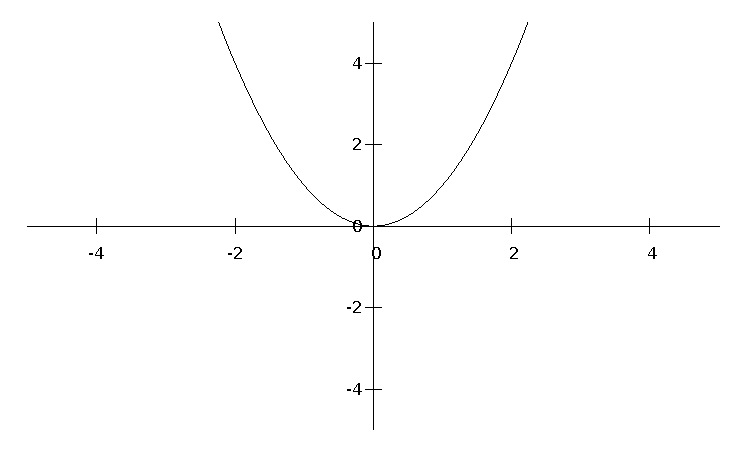
\includegraphics[width=1\textwidth]{graphics/01/01.pdf}
            \end{column}
            \begin{column}{.5\textwidth}
                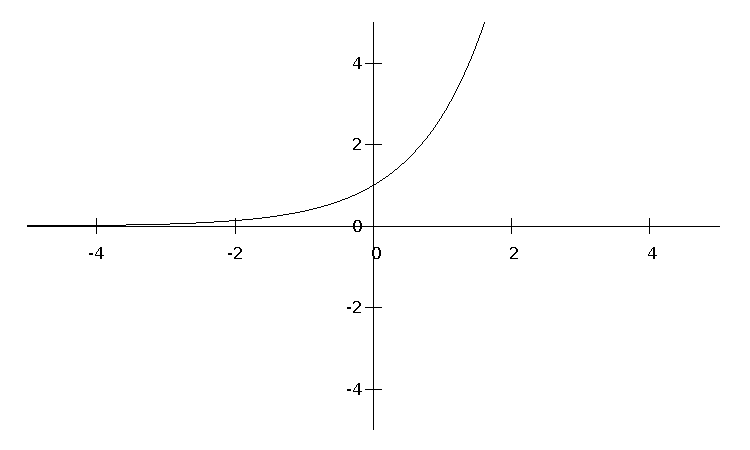
\includegraphics[width=1\textwidth]{graphics/01/02.pdf}
            \end{column}
        \end{columns}
        \begin{columns}
            \begin{column}{.5\textwidth}
                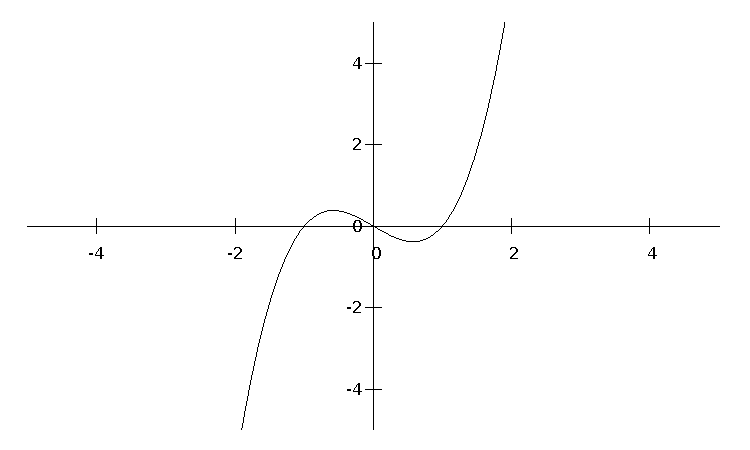
\includegraphics[width=1.\textwidth]{graphics/01/03.pdf}
            \end{column}
            \begin{column}{.5\textwidth}
                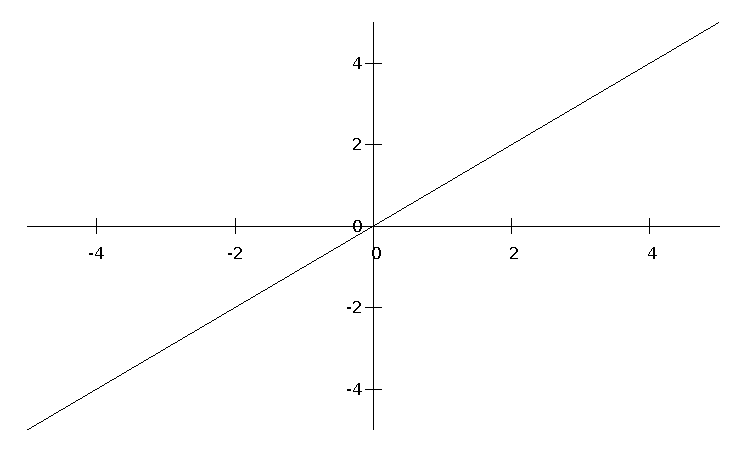
\includegraphics[width=1.\textwidth]{graphics/01/04.pdf}
            \end{column}
        \end{columns}
    \end{frame}
    \begin{frame}{Funktionen}
        \begin{alertblock}{Vorsicht}
            Unbedingt den Definitionsbereich einer Funktion beachten. Die Normalparabel ist im Bereich der komplexen Zahlen surjektiv!
        \end{alertblock}
    \end{frame}
    \begin{frame}{Übungsaufgabe}
        \begin{exampleblock}{Winter 2010/2011, Aufgabe 1.2}
            Es sei $A$ die Menge aller Kinobesucher in einer Vorstellung und $B$ die Menge aller Sitzplätze. Die Abbildung $f$ ordnet den Kinobesuchern die Sitzplätze zu: $ f: A \rightarrow B $
            \begin{itemize}
                \item Was bedeutet es im Kino, wenn $f$ linkstotal, linkseindeutig, rechtstotal, rechtseindeutig ist?
                \item Was wünschen sich die Kinobesucher: Eine injektive, surjektive oder bijektive Abbildung auf die Sitzplätze? Was wünscht sich der Besitzer?
                \item In dieser Teilaufgabe nehmen wir an, 6 Kinobesucher besuchten ein Kino mit 8 Plätzen. Zeichnen Sie eine injektive Abbildung $f$. Wie viele injektive Abbildungen gibt es? 
            \end{itemize}
        \end{exampleblock}
    \end{frame}

\section{Mengenlehre}
	\begin{frame}{Mengenlehre}
		\begin{block} {Definition Menge}
			Eine Menge ist eine beliebig große Ansammlung an Elementen\\
			$\Rightarrow$ es existieren Mengen ohne, endlich vielen und unendlich vielen Elementen.
		\end{block}

		\begin{block}{Schreibweiße von Mengen}
			Sei $M$ eine Menge bestehend aus den Elementen $0, 1, 2$, dann schreiben wir:\\
            \begin{align*}
                M = \left\{0, 1, 2\right\}
            \end{align*}
			Außerdem gilt: $0, 1, 2 \in M$
		\end{block}
	\end{frame}

	\begin{frame}{Besonderheiten}
		\begin{itemize}
			\item Die Reihenfolge der Elemente in einer Menge ist egal.\\
				Da $x,y \in \{x,y\}$ aber auch $x,y \in \{y,x\}$\\
				$\Rightarrow \{x,y\} = \{y,x\}$
			\pause
			\item Mehrfaches Vorkommen von Elementen ist auch egal.\\
				$\Rightarrow \{a, b, b, 3\} = \{a, b, 3\}$
		\end{itemize}
	\end{frame}

	\begin{frame}{Besondere Mengen}
		\begin{itemize}
			\item Die Leere Menge: $\emptyset = \{\}$
			\pause
			\item Die Nat\"urlichen Zahlen ohne 0: $\mathbb{N}_+ = \{1,2,3,...\}$
			\pause
			\item Die Nat\"urlichen Zahlen mit 0: $\mathbb{N}_0 = \{0,1,2,3,...\}$
			\pause
			\item Ganze Zahlen von 0 bis n-1: $\mathbb{G}_n = \{0,1,2,...,n-1\}$
		\end{itemize}
	\end{frame}

	\begin{frame}{Mengenoperationen}
		\begin{block}{Vereinigung von Mengen $\cup$}
			Sei $A = \{0,1,2\}$ und $B = \{a,b,c\}$\\
			Dann ist die Vereinigung der Mengen $A$ und $B$:\\
			$A \cup B = \{0,1,2\} \cup \{a,b,c\} = \{0,1,2,a,b,c\}$\\
			Alle Elemente aus $A$ und $B$ liegen somit in $A \cup B$

		\end{block}
		\pause

		\begin{block}{Durchschnitt von Mengen $\cap$}
			Sei $A = \{0,1,2\}$ und $B = \{1,2,3,4,a\}$\\
			Dann ist der Durchschnitt der Mengen $A$ und $B$:\\
			$A \cap B = \{0,1,2\} \cap \{1,2,3,4,a\} = \{1, 2\}$\\
			Im Durchschnitt liegen somit nur Elemente, die sowohl in $A$ und in $B$ liegen.
		\end{block}
	\end{frame}

	\begin{frame}{Aufgabenteil 1}
		Gegeben seien die Mengen $A$, $B$, $C$ und $D$, mit:
        \begin{align*}
		    A = \{1,3,5,9\}\\
		    B = \{1,2,4,8\}\\
		    C = \{x,d,1,2,3,4,9\}\\
		    D = \{a,c,d,x\}
		\end{align*}
		
		Die Menge $M$ sei definiert durch:\\
		\begin{align*}
			M = \Big(\big(D \cap C\big)\cup\big((C \cap B)\cup(A \cap C)\big)\Big) \setminus (A \cap B)
		\end{align*}
		
		Welche Elemente enth\"alt die Menge M?	
			
		Antwort: 
		\visible<2>{$M= \{d,x,2,3,4,9\}$}
 	\end{frame}
 	
 	
 	
 	\begin{frame} {Mengenraten}
     	\begin{center}
     		\begin{tabular}{c|c}
     		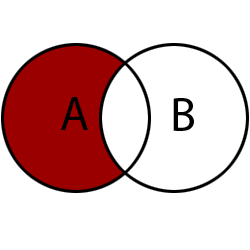
\includegraphics[scale=.35]{graphics/01/menge1.png} &
		    \visible<2-4>{
\includegraphics[scale=.35]{graphics/01/menge2.png}}
     		 \\
     		\hline 
     		\visible<3-4>{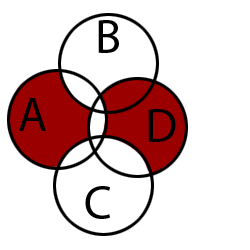
\includegraphics[scale=.35]{graphics/01/menge3.png}}
     		 & 		
     		\visible<4>{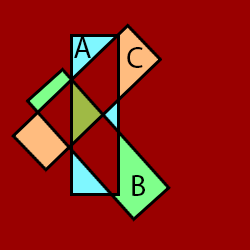
\includegraphics[scale=.35]{graphics/01/menge4.png}} 			\\
     		\end{tabular} 
     	\end{center}
 	\end{frame}

\end{document}
